\documentclass[aspectratio=169, 10pt]{beamer}

\usetheme{metropolis}
\metroset{block=fill, numbering=fraction, progressbar=frametitle}

\usepackage[utf8]{inputenc}
\usepackage[T1]{fontenc}
\usepackage[spanish]{babel}
\usepackage{graphicx}
\usepackage{amsmath, amssymb}
\usepackage{booktabs}
\usepackage{xcolor}
\usepackage{siunitx}

\graphicspath{{../ej1/results/pca/}{../ej1/results/oja/}{../ej1/results/kohonen/}}

\definecolor{accent}{HTML}{0F4C81}
\setbeamercolor{frametitle}{bg=accent}
\setbeamercolor{progress bar}{fg=accent}

\title{Aprendizaje No Supervisado}
\subtitle{Ejercicio 1 --- Europa: PCA, Regla de Oja y Red de Kohonen}
\author{TP4 -- Sistemas de Inteligencia Artificial}
\institute{ITBA --- 2026}
\date{\today}

\begin{document}

\maketitle

% ============================================================
% BLOQUE 0: SETUP
% ============================================================

\begin{frame}{El problema}
  \begin{columns}[T]
    \begin{column}{0.55\textwidth}
      \textbf{Dataset:} \texttt{europe.csv} --- 28 paises europeos $\times$ 7 variables numericas.
      \vspace{0.3em}
      \begin{itemize}
        \item Area (km$^2$)
        \item GDP (PIB per capita)
        \item Inflation (\%)
        \item Life.expect (anios)
        \item Military (presupuesto)
        \item Pop.growth (\%)
        \item Unemployment (\%)
      \end{itemize}
      \vspace{0.5em}
      \textbf{Objetivo:} descubrir estructura --- relaciones entre variables, agrupamiento de paises --- \alert{sin etiquetas}.
    \end{column}
    \begin{column}{0.45\textwidth}
      \textbf{Tres tecnicas, una historia:}
      \begin{itemize}
        \item \textbf{PCA (libreria)}: reduccion de dimensionalidad por autovalores.
        \item \textbf{Oja}: PC1 iterativa, sin resolver autovalores explicitamente.
        \item \textbf{Kohonen / SOM}: mapeo a grilla 2D conservando topologia.
      \end{itemize}
    \end{column}
  \end{columns}
\end{frame}

\begin{frame}{Las escalas son muy distintas}
  \begin{columns}[T]
    \begin{column}{0.55\textwidth}
      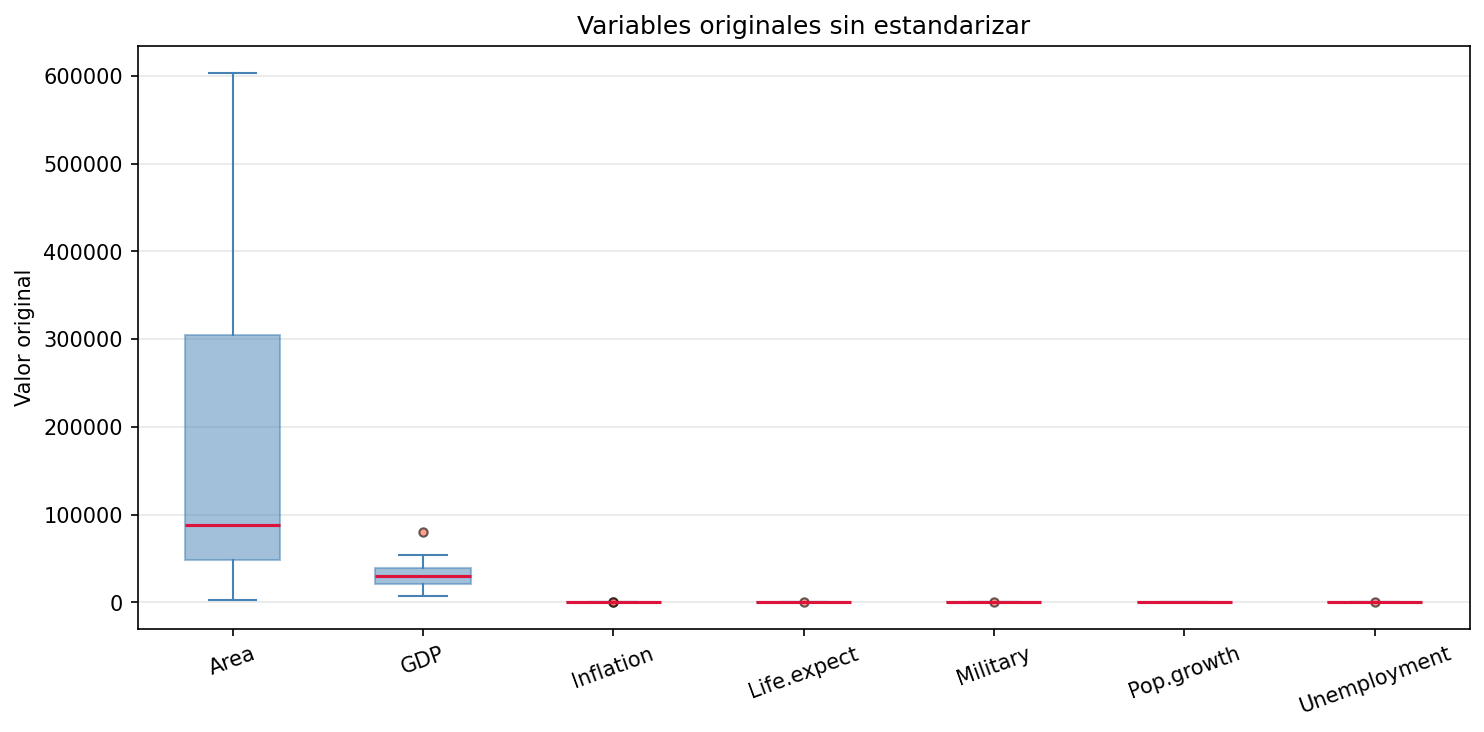
\includegraphics[width=\linewidth]{boxplot_raw}
    \end{column}
    \begin{column}{0.45\textwidth}
      \textbf{Sin estandarizar}:
      \begin{itemize}
        \item \texttt{Area} domina ($\sim 10^5$).
        \item \texttt{GDP} en otro orden de magnitud ($\sim 10^4$).
        \item \texttt{Inflation}, \texttt{Life.expect}, \texttt{Military}, \texttt{Pop.growth}, \texttt{Unemployment}: $\sim 10^0$--$10^1$.
      \end{itemize}
      \vspace{0.7em}
      \textbf{Consecuencia:} la varianza esta dominada por la escala, no por la informacion. Aplicar PCA o medir distancias asi seria \alert{enganioso}.
    \end{column}
  \end{columns}
\end{frame}

% ============================================================
% BLOQUE A: PCA
% ============================================================

\section{PCA con libreria}

\begin{frame}{Estandarizacion}
  \begin{columns}[T]
    \begin{column}{0.55\textwidth}
      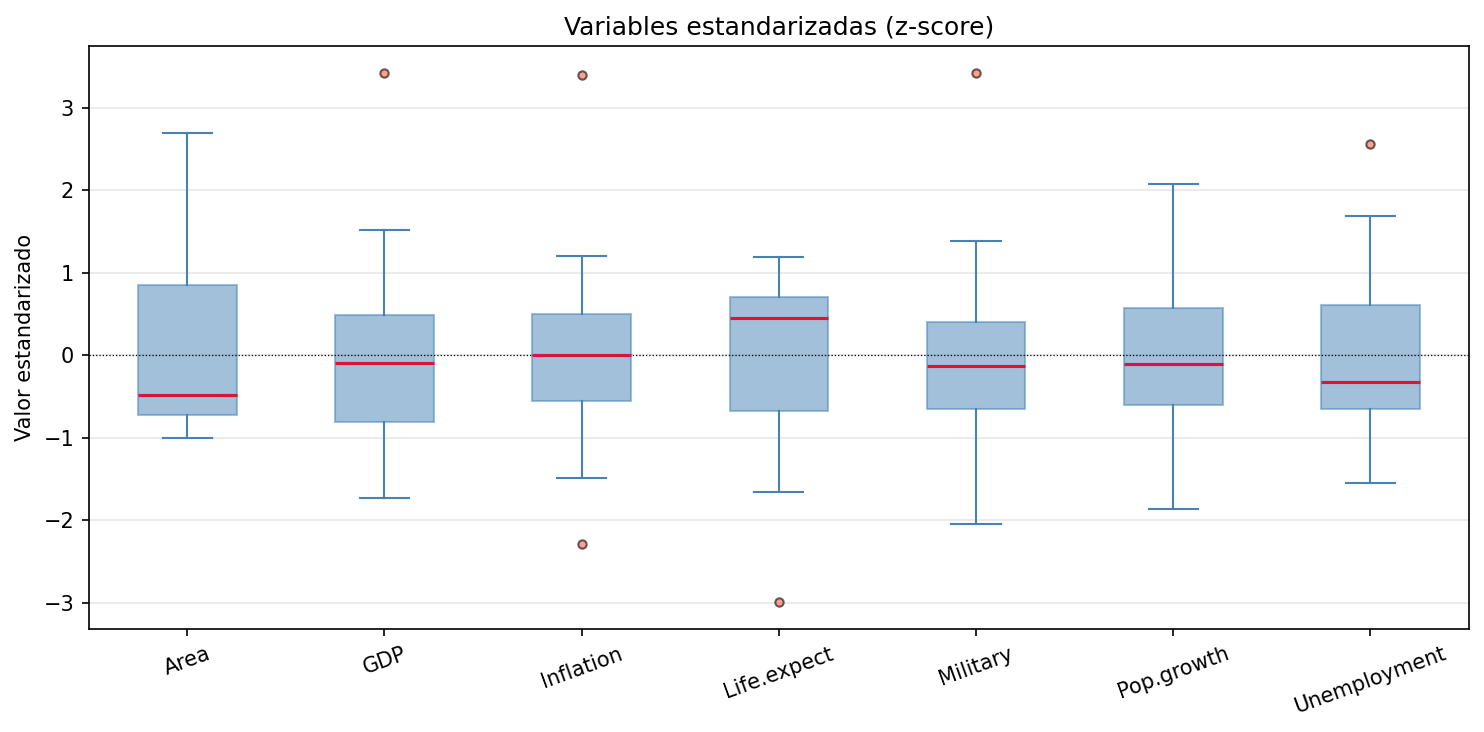
\includegraphics[width=\linewidth]{boxplot_standardized}
    \end{column}
    \begin{column}{0.45\textwidth}
      \textbf{Z-score}:
      \[ \tilde{X}_j = \frac{X_j - \bar{X}_j}{s_j} \]
      Cada variable queda con media~0 y varianza~1. Todas las variables son ahora \alert{comparables}.
      \vspace{0.5em}

      \textbf{Equivalencia clave}: aplicar PCA sobre los datos estandarizados $\equiv$ aplicar PCA sobre la matriz de \alert{correlacion} (no de covarianza).
    \end{column}
  \end{columns}
\end{frame}

\begin{frame}{Hay redundancia: tiene sentido hacer PCA}
  \begin{columns}[c]
    \begin{column}{0.6\textwidth}
      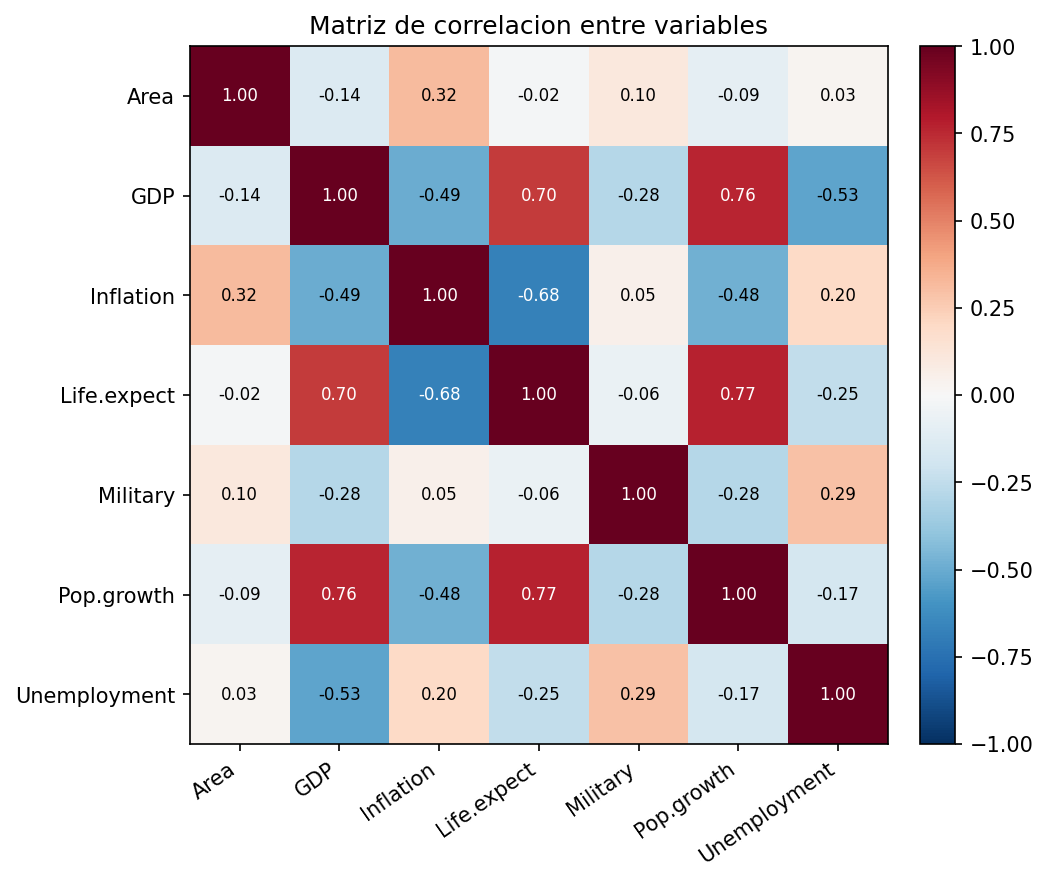
\includegraphics[width=\linewidth]{correlation_heatmap}
    \end{column}
    \begin{column}{0.4\textwidth}
      Varias variables estan fuertemente correlacionadas:
      \begin{itemize}
        \item \texttt{GDP} y \texttt{Life.expect} ($r = +0.74$).
        \item \texttt{Inflation} con varias ($r$ negativos).
        \item \texttt{Pop.growth} con \texttt{GDP} y \texttt{Life.expect} ($r > 0.4$).
      \end{itemize}
      Si no hubiera correlacion, no tendria sentido hacer PCA.
    \end{column}
  \end{columns}
\end{frame}

\begin{frame}{Cuanta informacion explica cada componente}
  \begin{columns}[c]
    \begin{column}{0.6\textwidth}
      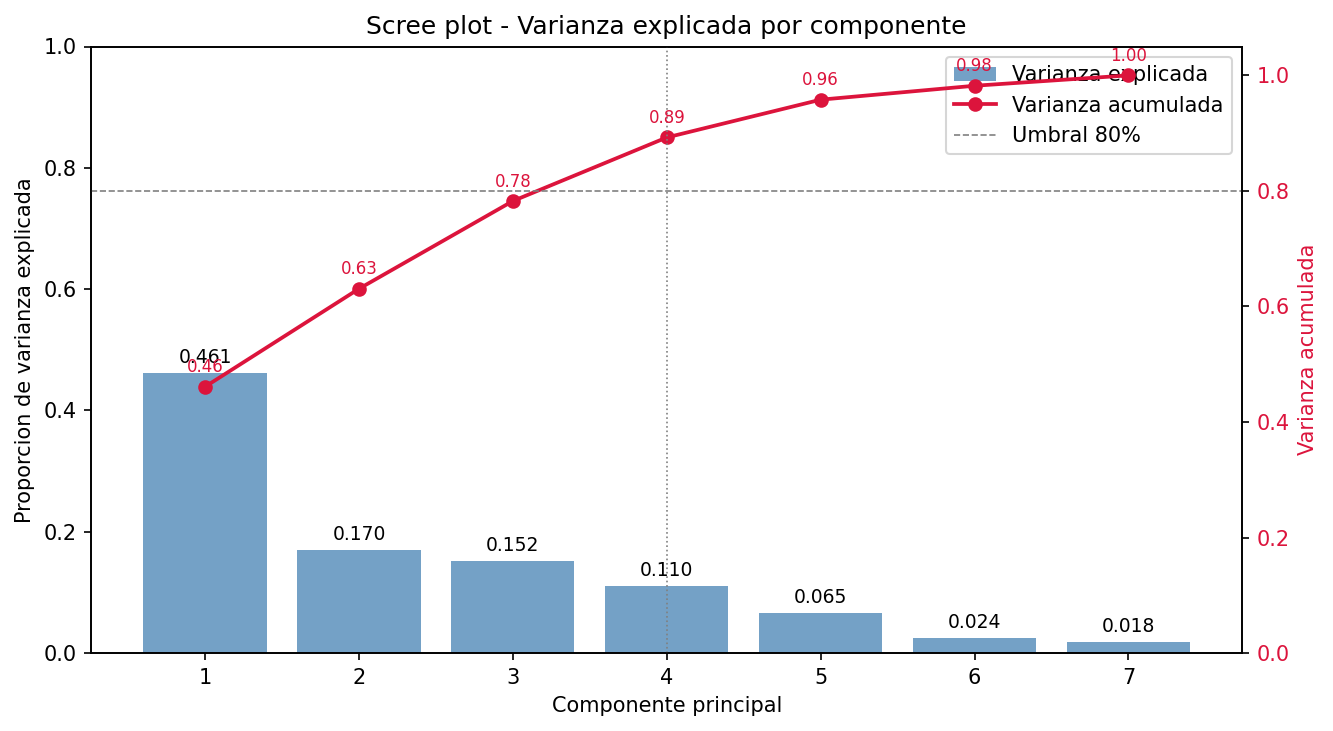
\includegraphics[width=\linewidth]{scree_plot}
    \end{column}
    \begin{column}{0.4\textwidth}
      \begin{itemize}
        \item \textbf{PC1}: 46.1\% de la varianza.
        \item \textbf{PC2}: 17.0\%.
        \item \textbf{PC3}: 15.2\%.
        \item \textbf{PC1+PC2+PC3}: 78.3\%.
        \item Hace falta una \textbf{4ta} componente para cruzar el 80\%.
      \end{itemize}
      \vspace{0.5em}
      Con 2 componentes ya capturamos $\sim$63\% --- suficiente para visualizar.
    \end{column}
  \end{columns}
\end{frame}

\begin{frame}{Cargas: que representa cada componente}
  \begin{columns}[c]
    \begin{column}{0.6\textwidth}
      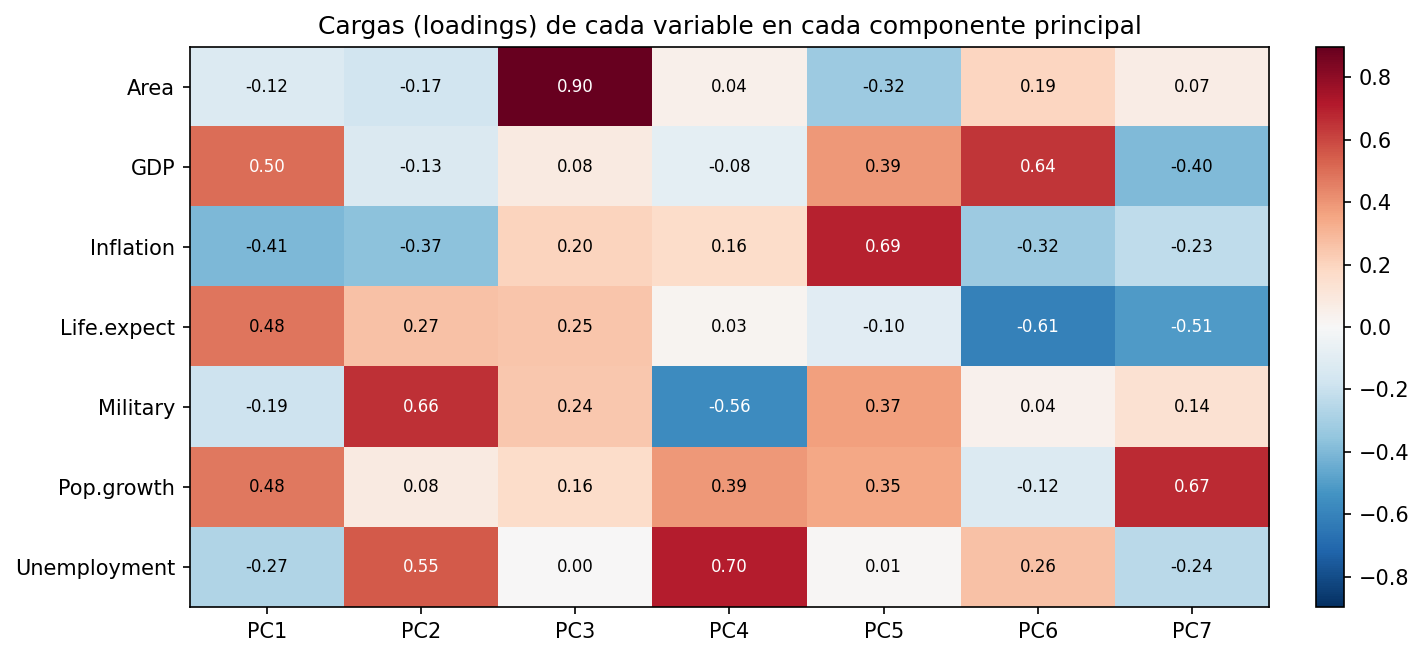
\includegraphics[width=\linewidth]{loadings_heatmap}
    \end{column}
    \begin{column}{0.4\textwidth}
      \textbf{PC1 -- ``Desarrollo''}\\
      $+$\texttt{GDP}, $+$\texttt{Life.expect}, $+$\texttt{Pop.growth},\\
      $-$\texttt{Inflation}, $-$\texttt{Unemployment}.
      \vspace{0.4em}

      \textbf{PC2 -- ``Crisis''}\\
      $+$\texttt{Military}, $+$\texttt{Unemployment} vs $-$\texttt{Inflation}.\\
      Captura Grecia / Espania / Croacia.
      \vspace{0.4em}

      \textbf{PC3 -- ``Tamanio''}\\
      Casi solo \texttt{Area} ($+0.90$).
    \end{column}
  \end{columns}
\end{frame}

\begin{frame}{Biplot PC1 vs PC2: agrupamientos}
  \centering
  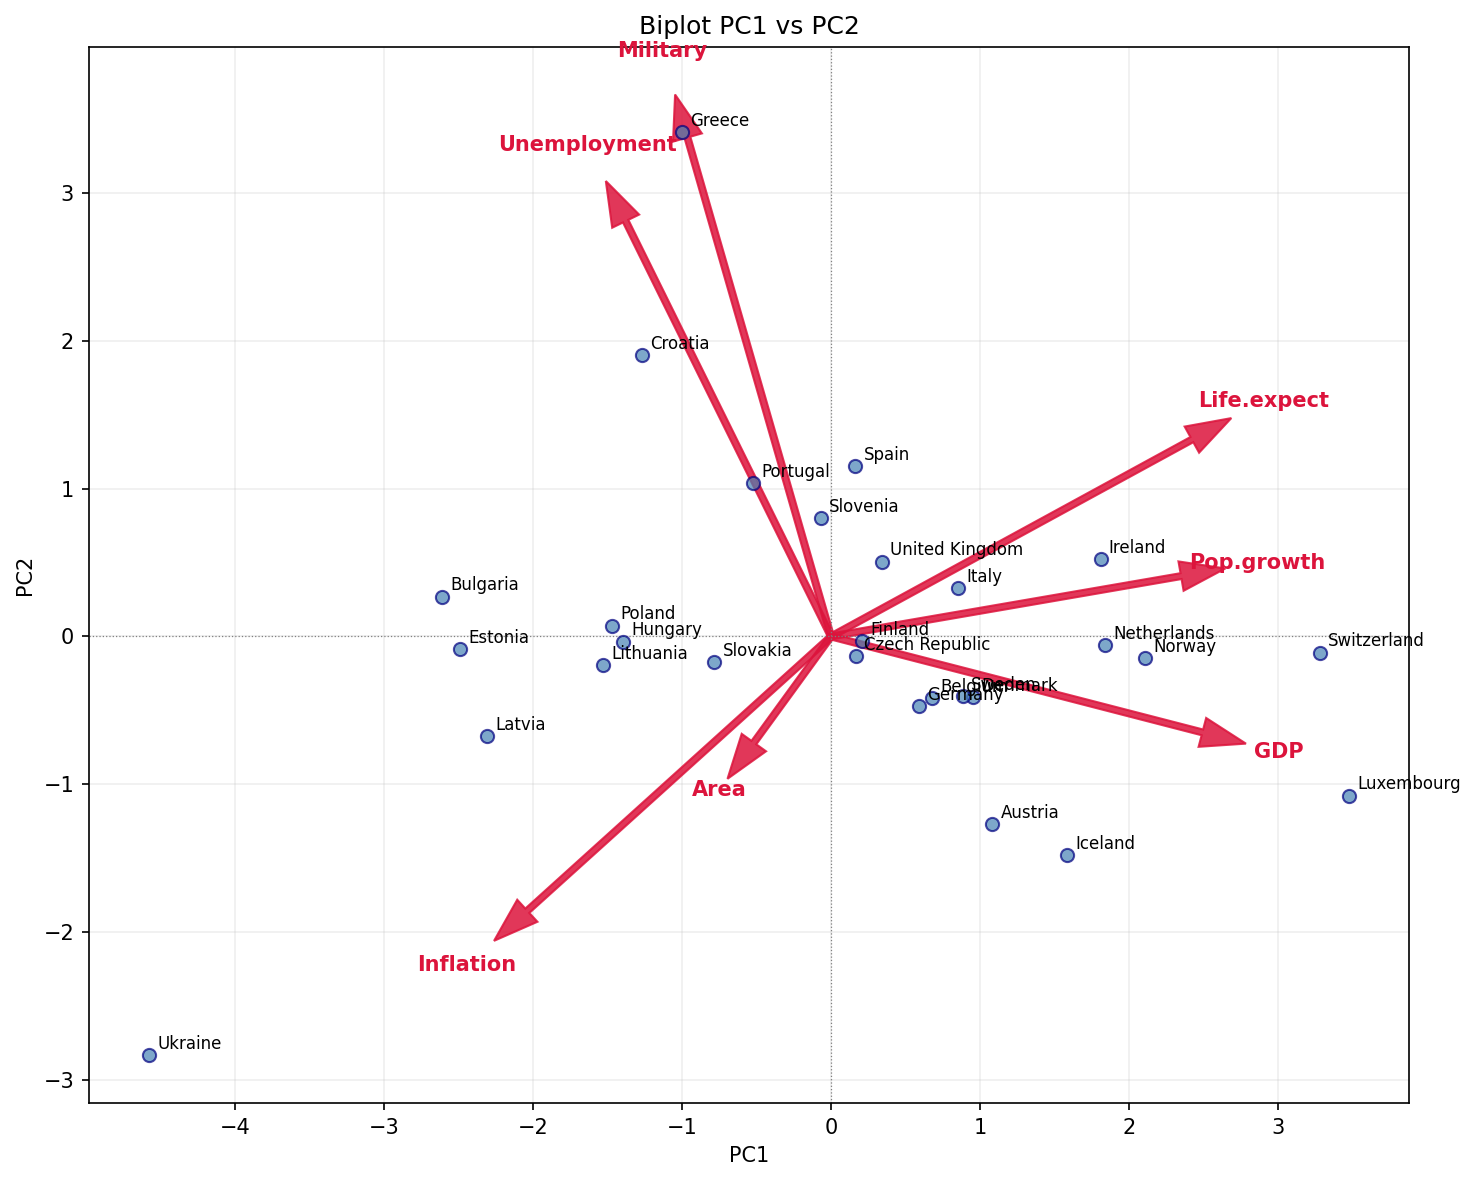
\includegraphics[height=0.85\textheight]{biplot_pc1_pc2}
\end{frame}

\begin{frame}{Ranking de paises segun PC1}
  \begin{columns}[T]
    \begin{column}{0.55\textwidth}
      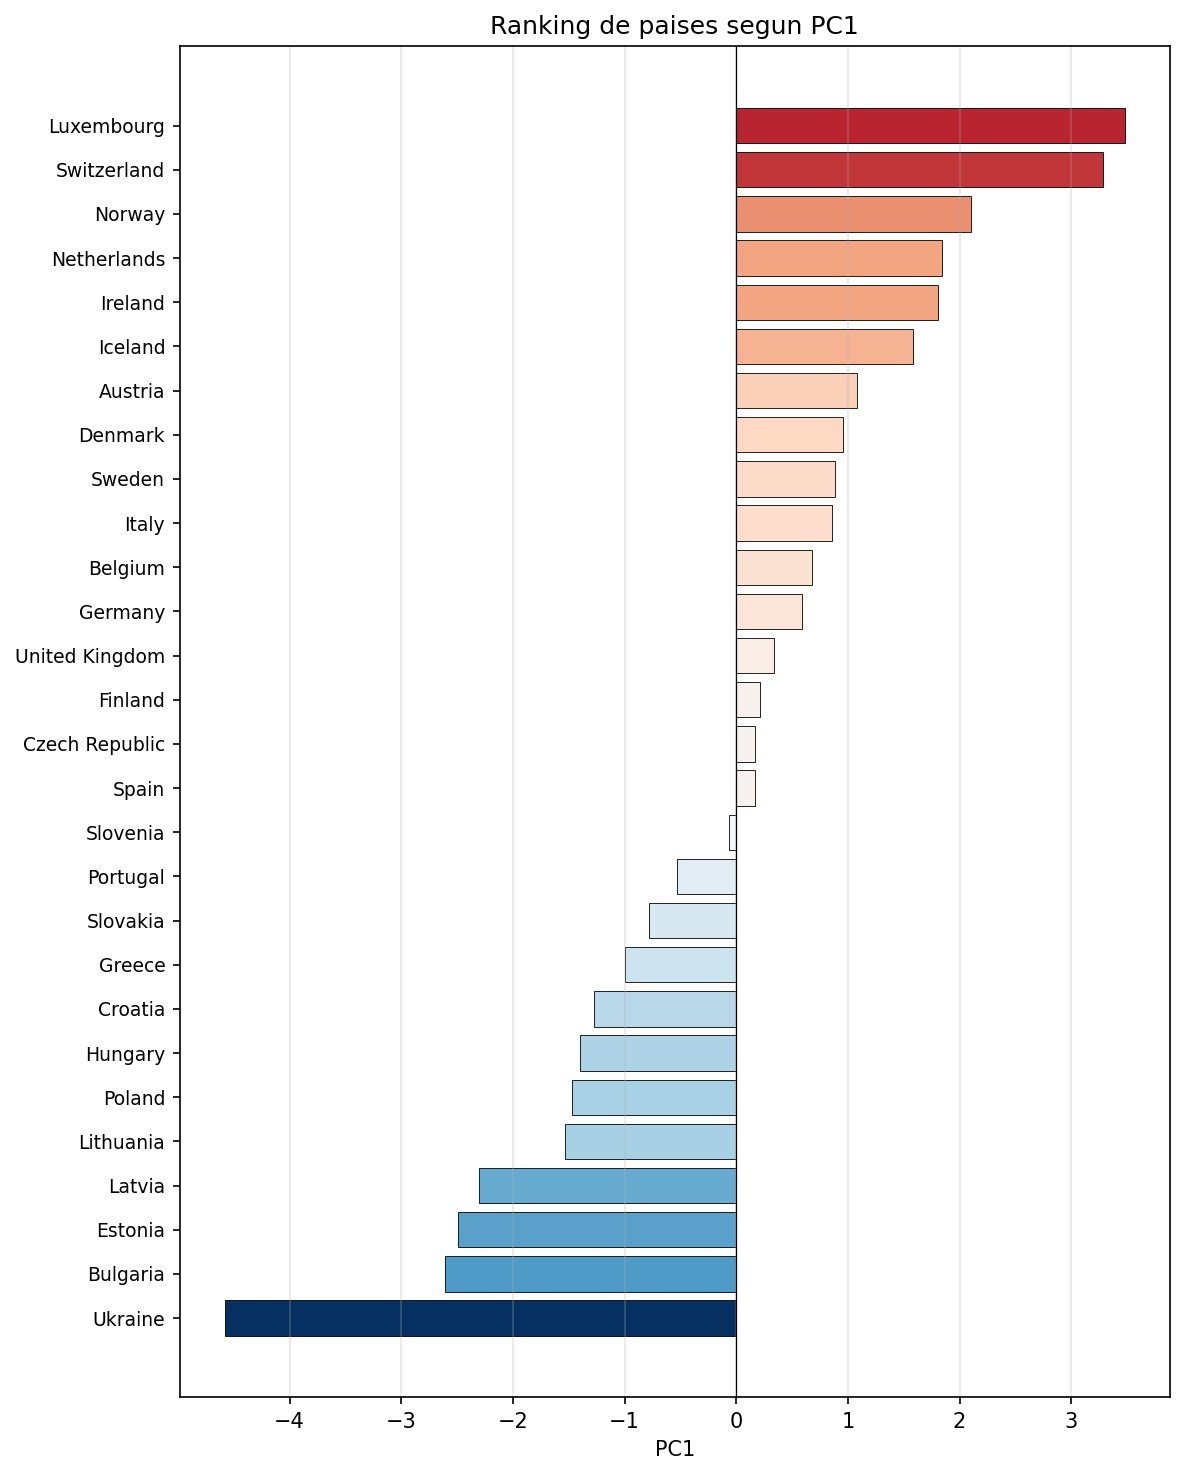
\includegraphics[height=0.85\textheight]{pc1_ranking}
    \end{column}
    \begin{column}{0.45\textwidth}
      PC1 ordena los paises por un \textbf{indice de desarrollo / bienestar}:
      \vspace{0.4em}
      \begin{itemize}
        \item \textbf{Top}: Luxembourg, Switzerland, Norway, Netherlands, Ireland.
        \item \textbf{Centro}: Italy, Belgium, Germany, UK.
        \item \textbf{Bottom}: Ukraine, Bulgaria, Estonia, Latvia.
      \end{itemize}
      \vspace{0.5em}
      Es la \alert{nueva variable sintetica} que mejor diferencia los paises del dataset.
    \end{column}
  \end{columns}
\end{frame}

\begin{frame}{PC2: dimension complementaria}
  \begin{columns}[T]
    \begin{column}{0.55\textwidth}
      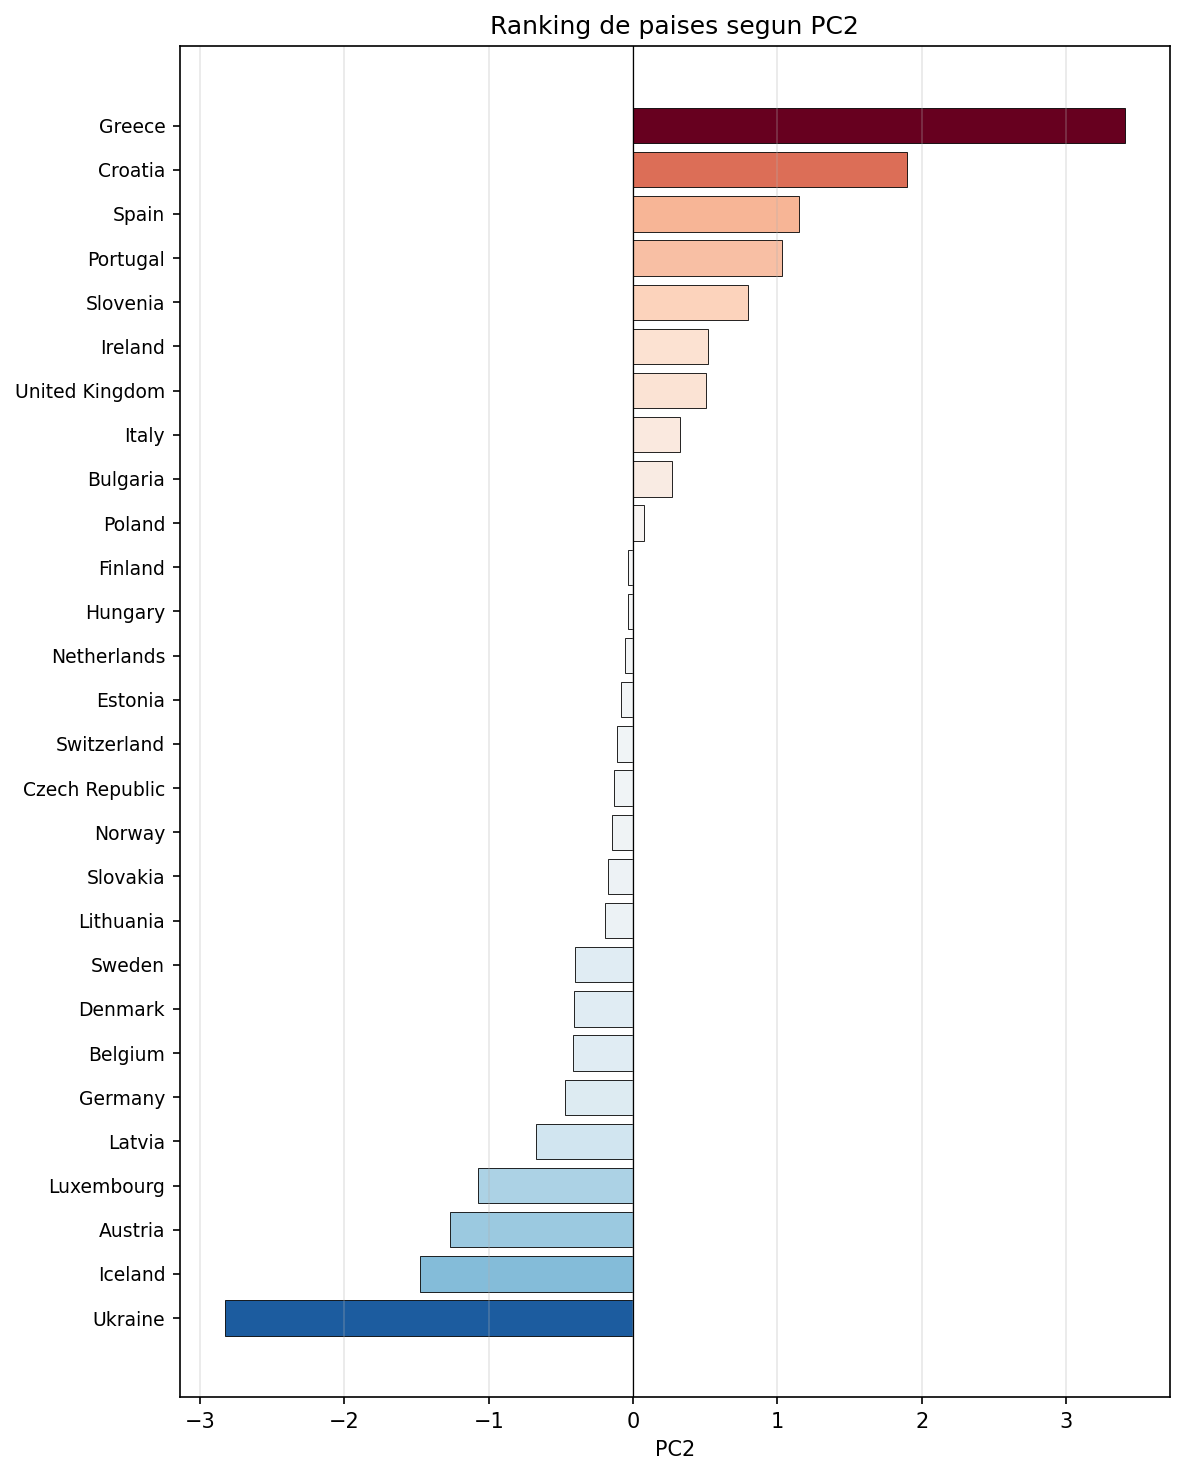
\includegraphics[height=0.85\textheight]{pc2_ranking}
    \end{column}
    \begin{column}{0.45\textwidth}
      PC2 captura un eje \textbf{ortogonal} a PC1:
      \vspace{0.4em}
      \begin{itemize}
        \item Arriba: Grecia, Croacia, Spain --- alta inestabilidad (Military / Unemployment).
        \item Abajo: Luxemburgo, Iceland, Austria --- estabilidad fiscal.
      \end{itemize}
      \vspace{0.5em}
      Algunos paises con PC1 medio (Spain) se separan claramente en PC2.
    \end{column}
  \end{columns}
\end{frame}

% ============================================================
% BLOQUE B: OJA
% ============================================================

\section{Regla de Oja}

\begin{frame}{Calcular PC1 sin resolver autovalores}
  \begin{columns}[T]
    \begin{column}{0.55\textwidth}
      \textbf{Idea}: un perceptron lineal con una neurona y la regla de actualizacion
      \[
      \Delta w = \eta \, y \, (x - y \, w), \quad y = w^T x
      \]
      \textbf{Por que funciona:}
      \begin{itemize}
        \item Hebbiano puro hace que $\|w\| \to \infty$.
        \item El termino $-y\,w$ normaliza implicitamente: $\|w\| \to 1$.
        \item $w$ converge al \alert{autovector del mayor autovalor} de la matriz de correlacion --- es la PC1.
      \end{itemize}
    \end{column}
    \begin{column}{0.45\textwidth}
      \textbf{Hiperparametros}:
      \begin{itemize}
        \item Inicializacion: $w_0 \sim \mathcal{U}(0,1)$, normalizada.
        \item $\eta = 10^{-3}$ constante.
        \item Epocas: 200.
        \item Datos: estandarizados (media~0, std~1).
      \end{itemize}
      \vspace{0.4em}
      Recomendaciones teoricas: estandarizar siempre y usar $\eta \leq 0.5$ o $10^{-3}$ pequenio.
    \end{column}
  \end{columns}
\end{frame}

\begin{frame}{Convergencia: $\|w\| \to 1$ y $w \to$ PC1}
  \centering
  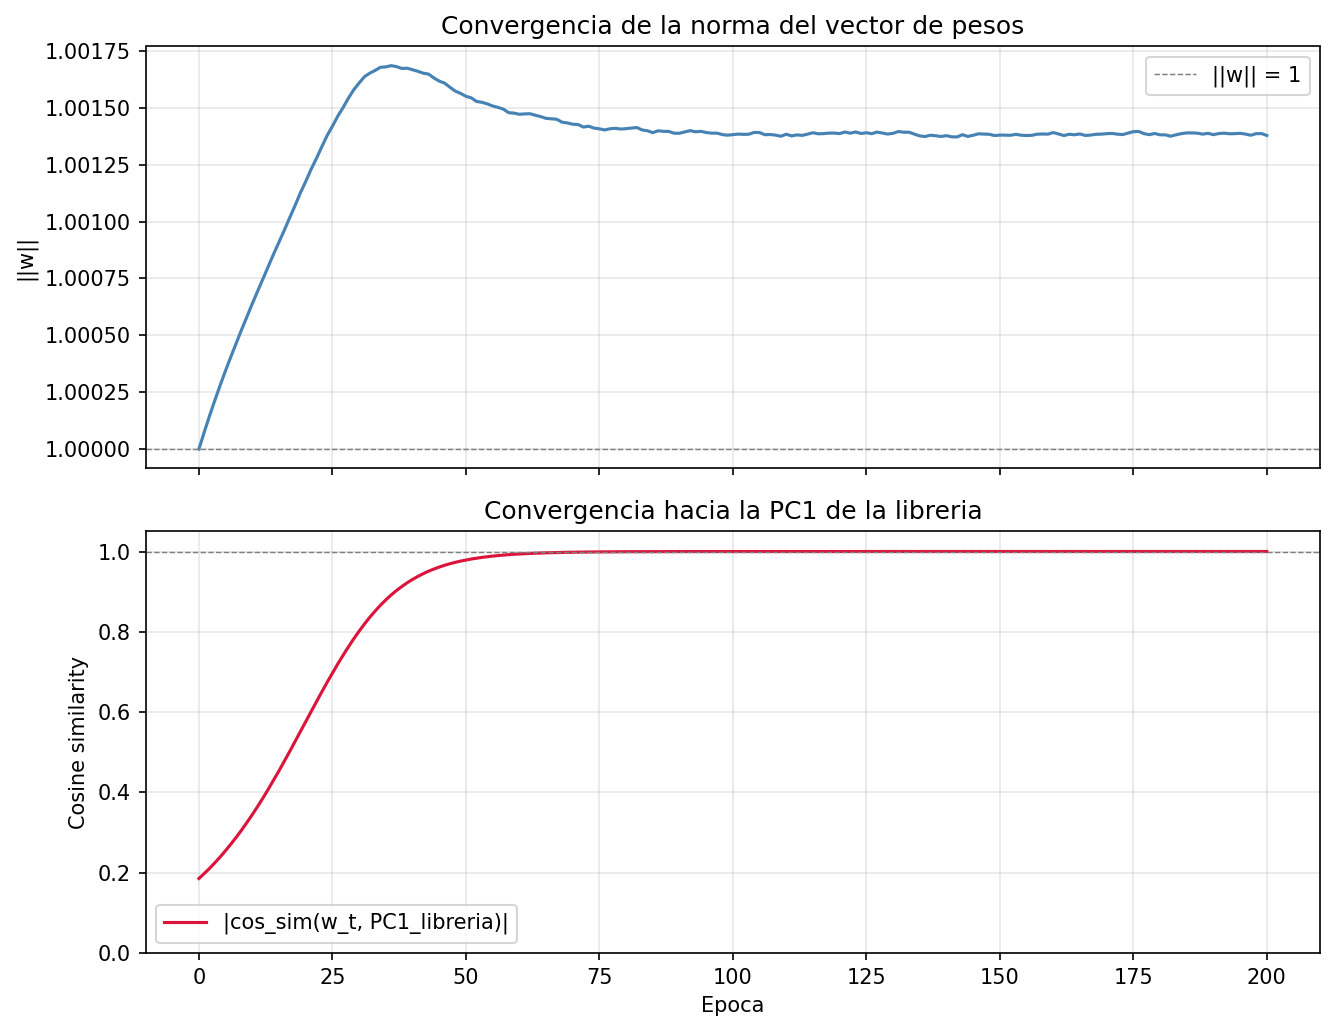
\includegraphics[height=0.85\textheight]{oja_convergence}
\end{frame}

\begin{frame}{Evolucion de las componentes de $w$}
  \centering
  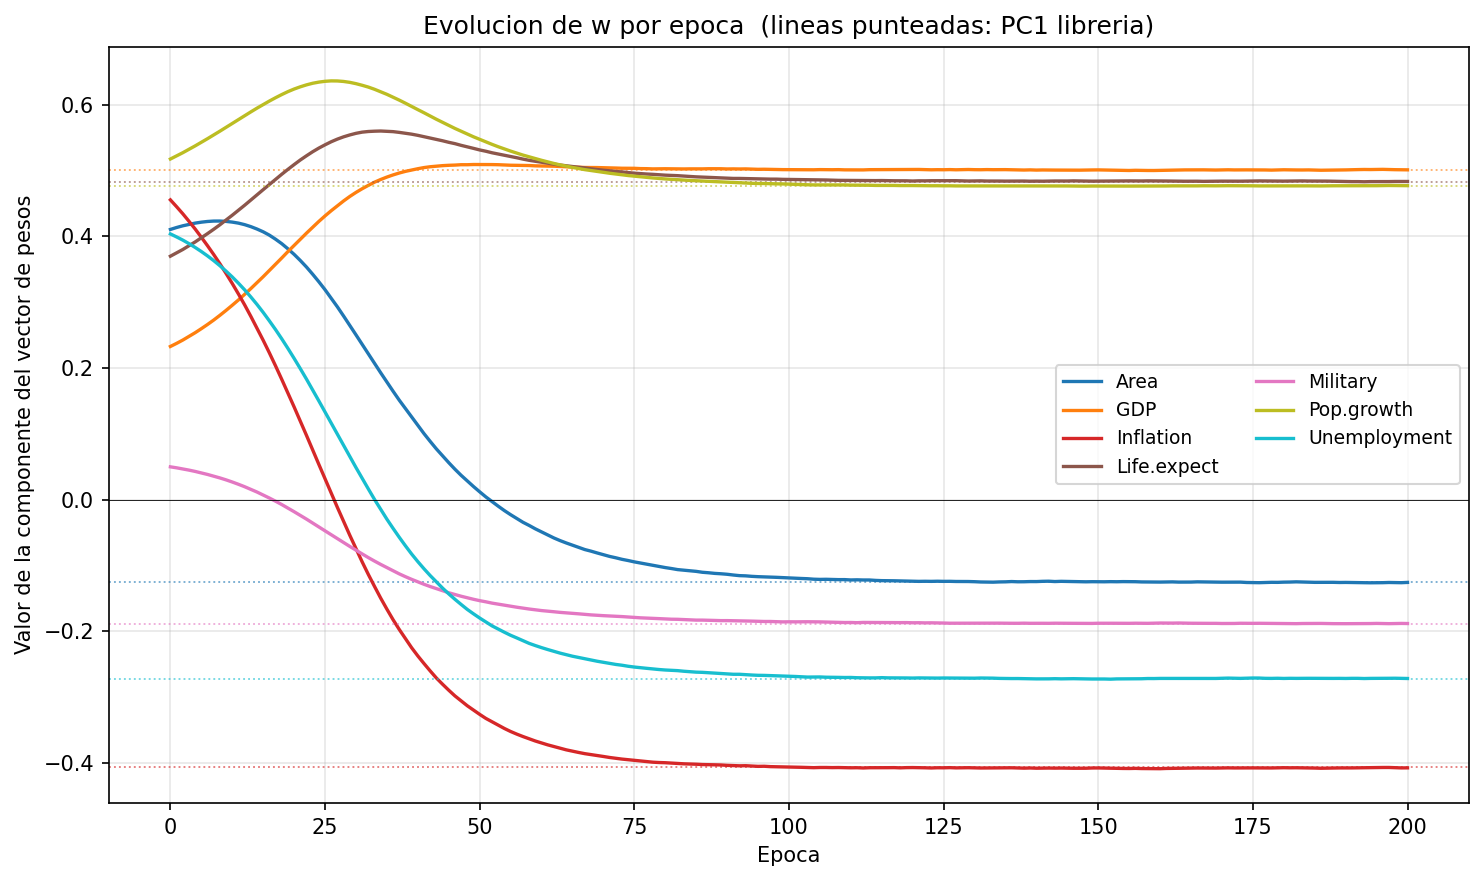
\includegraphics[height=0.85\textheight]{oja_weights_evolution}
\end{frame}

\begin{frame}{Comparacion con la libreria: cargas}
  \centering
  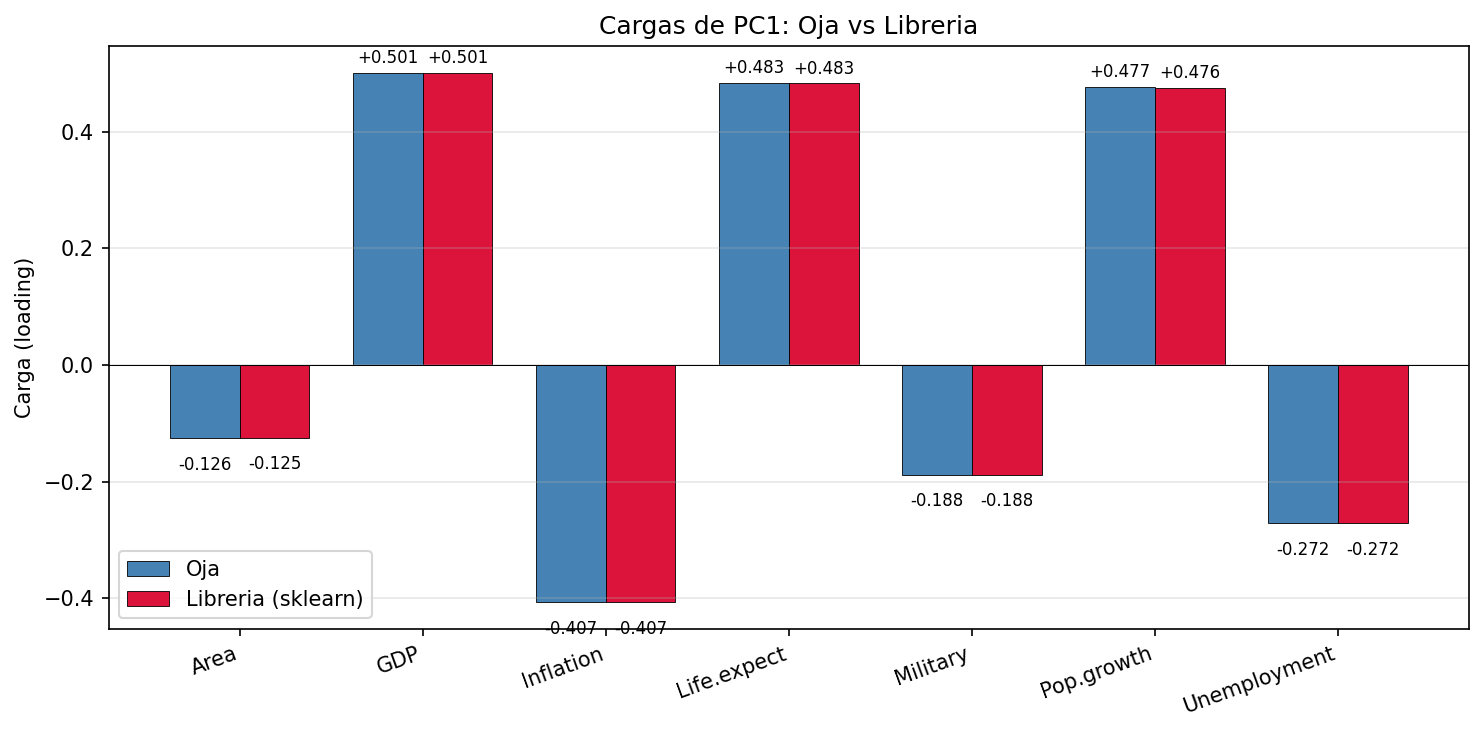
\includegraphics[height=0.85\textheight]{oja_vs_library_loadings}
\end{frame}

\begin{frame}{Comparacion: scores por pais}
  \begin{columns}[c]
    \begin{column}{0.55\textwidth}
      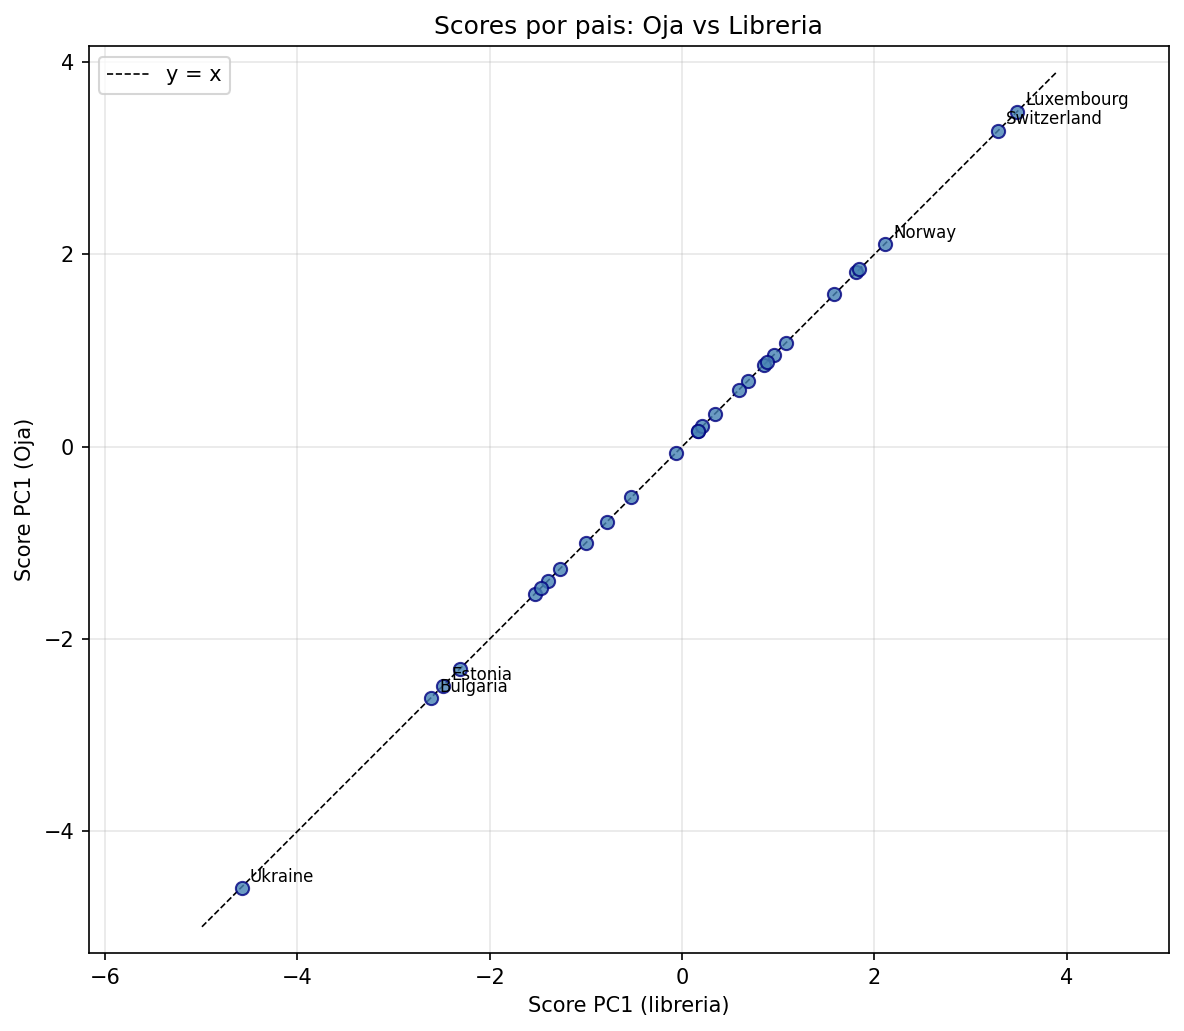
\includegraphics[width=\linewidth]{oja_vs_library_scores}
    \end{column}
    \begin{column}{0.45\textwidth}
      \textbf{Metricas de coincidencia}:
      \begin{itemize}
        \item Cosine similarity cargas: $+0.99999943$.
        \item Max abs error cargas: $0.00126$.
        \item RMSE cargas: $0.00066$.
        \item Pearson scores: $+0.99999986$.
        \item \alert{Spearman ranking: $+1.0$}.
        \item $\|w_{\text{Oja}}\| = 1.0014$.
      \end{itemize}
      \vspace{0.4em}
      Oja recupera la PC1 con error numerico despreciable, sin haber resuelto un solo problema de autovalores.
    \end{column}
  \end{columns}
\end{frame}

% ============================================================
% BLOQUE C: KOHONEN
% ============================================================

\section{Red de Kohonen / SOM}

\begin{frame}{Mapeo no-lineal a una grilla 2D}
  \begin{columns}[T]
    \begin{column}{0.55\textwidth}
      \textbf{Arquitectura}: grilla $k \times k$ de neuronas, cada una con peso $W_j \in \mathbb{R}^n$.
      \vspace{0.4em}

      \textbf{Algoritmo competitivo}:
      \begin{enumerate}
        \item Para cada muestra $x$, encontrar la neurona ganadora $\hat{k} = \arg\min_j \|x - W_j\|$.
        \item Actualizar a las neuronas dentro del radio $R(t)$ en la grilla:
        \[ W_j \leftarrow W_j + \eta(t) \, (x - W_j) \]
        \item $\eta(t)$ y $R(t)$ decrecen con el tiempo.
      \end{enumerate}
    \end{column}
    \begin{column}{0.45\textwidth}
      \textbf{Hiperparametros}:
      \begin{itemize}
        \item Grilla $4 \times 4$ (16 neuronas; $\sim$2 paises/neurona).
        \item $\eta(t)$: $0.5 \to 0.01$ lineal.
        \item $R(t)$: $2 \to 1$ lineal.
        \item 500 epocas (14000 iteraciones).
        \item Inicializacion: muestras del dataset.
        \item Distancia: euclidea.
      \end{itemize}
    \end{column}
  \end{columns}
\end{frame}

\begin{frame}{Convergencia}
  \begin{columns}[c]
    \begin{column}{0.65\textwidth}
      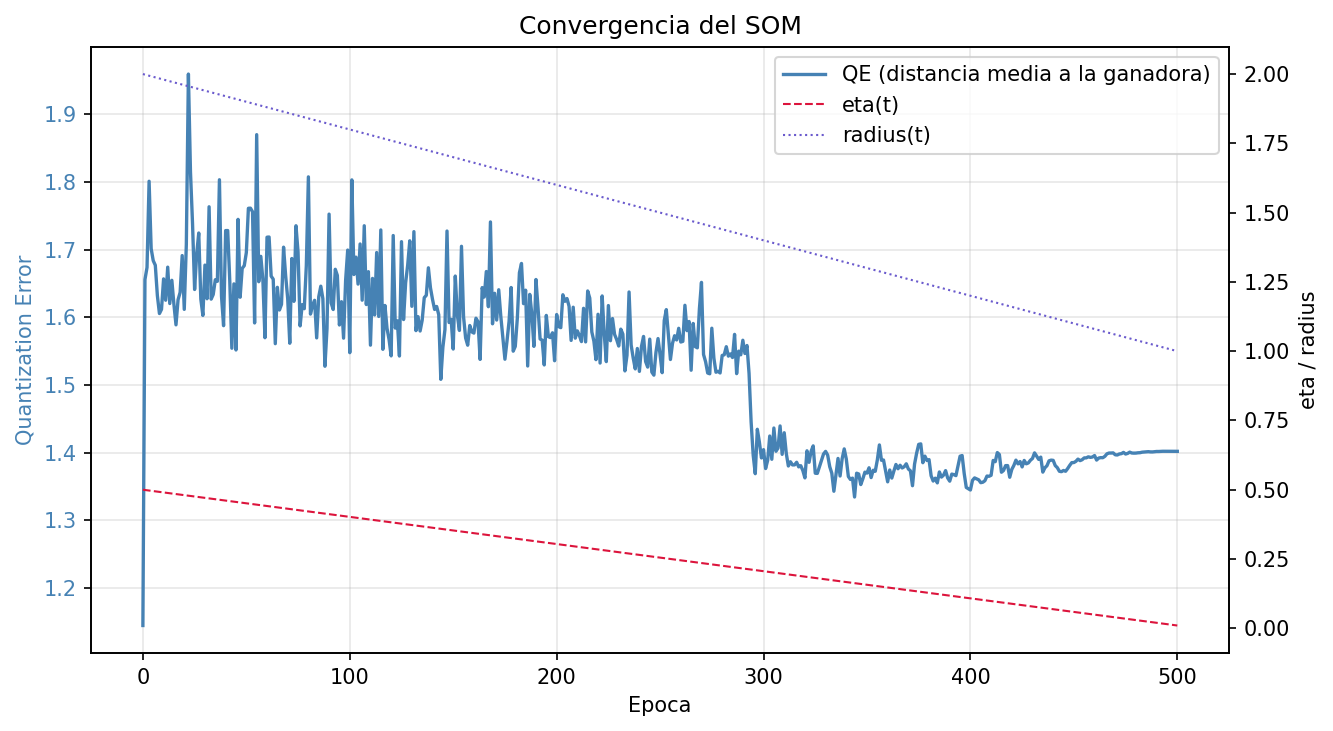
\includegraphics[width=\linewidth]{kohonen_convergence}
    \end{column}
    \begin{column}{0.35\textwidth}
      \textbf{Lectura}:
      \begin{itemize}
        \item Las primeras epocas son ``ruidosas'': el radio amplio mezcla todo.
        \item Hacia la epoca 290 el radio se acerca a 1 --- transicion de fase: solo se actualizan ganadora y vecinos directos.
        \item QE se estabiliza ($\sigma_{\text{rel}} = 4.8 \times 10^{-4}$ en las ultimas 20 epocas).
      \end{itemize}
    \end{column}
  \end{columns}
\end{frame}

\begin{frame}{Mapa de paises}
  \centering
  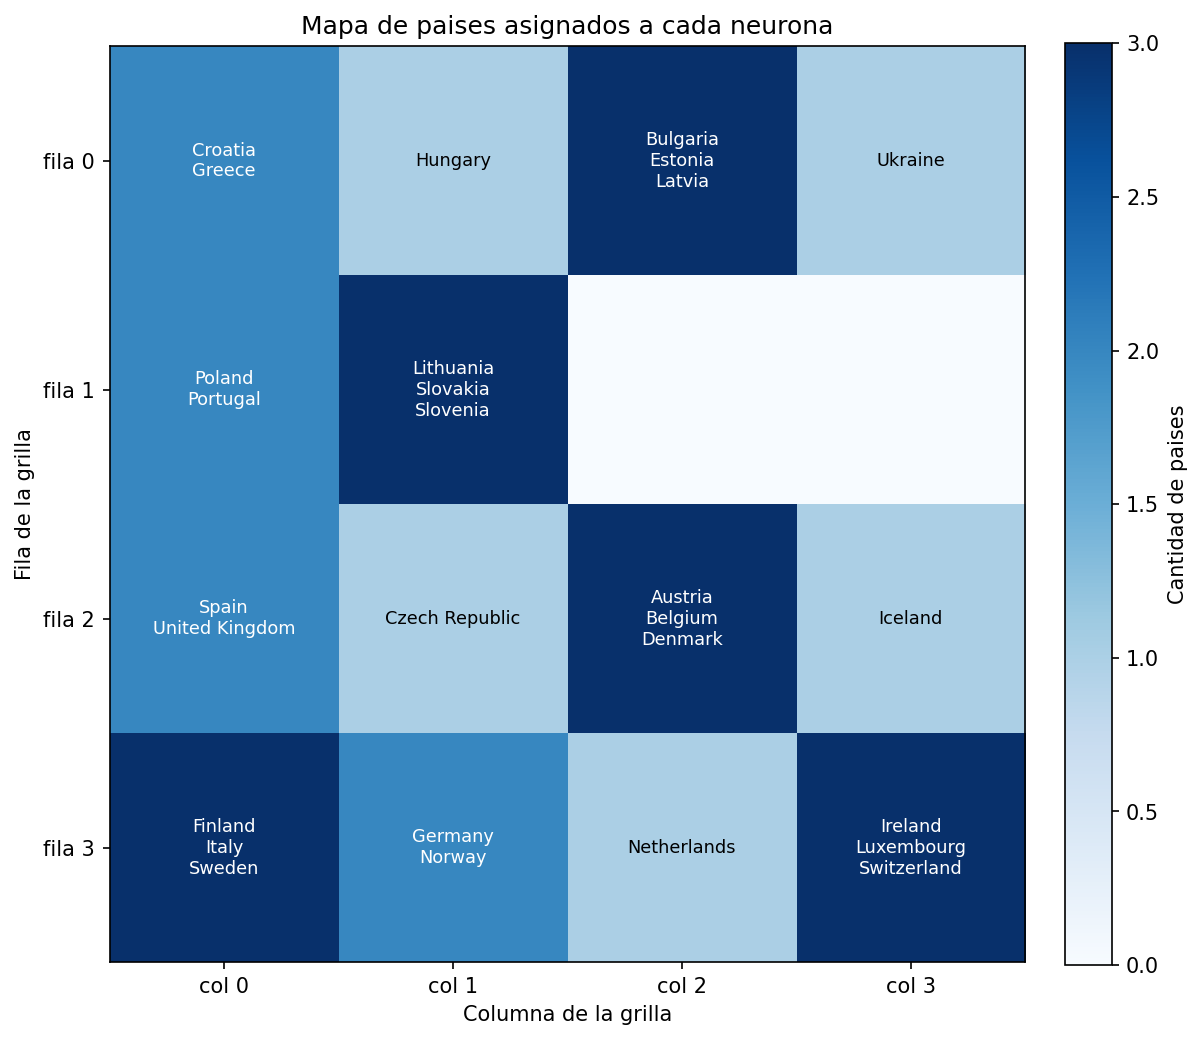
\includegraphics[height=0.85\textheight]{kohonen_country_map}
\end{frame}

\begin{frame}{Matriz U: fronteras entre clusters}
  \begin{columns}[c]
    \begin{column}{0.55\textwidth}
      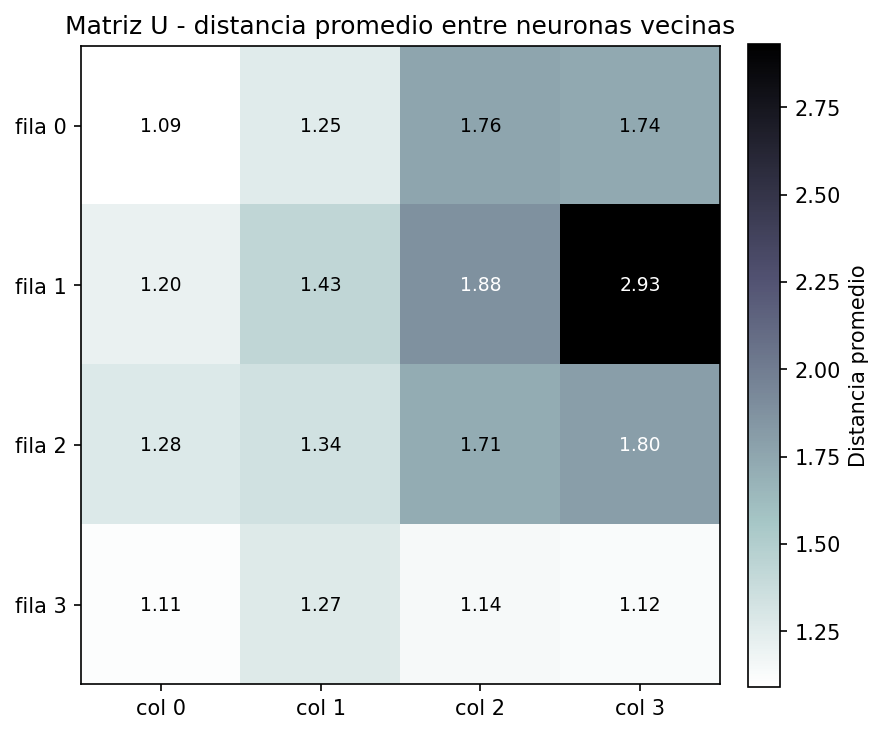
\includegraphics[width=\linewidth]{kohonen_u_matrix}
    \end{column}
    \begin{column}{0.45\textwidth}
      Distancia promedio de cada neurona a sus 8 vecinos:
      \begin{itemize}
        \item \textbf{Claro}: neuronas similares (clusters).
        \item \textbf{Oscuro}: fronteras.
      \end{itemize}
      \vspace{0.4em}
      La neurona en \texttt{(1,3)} es la frontera entre Ucrania (esquina (0,3)) y el resto --- distancia 2.93 --- es el outlier mas marcado del dataset.
    \end{column}
  \end{columns}
\end{frame}

\begin{frame}{Cantidad de paises por neurona}
  \begin{columns}[c]
    \begin{column}{0.55\textwidth}
      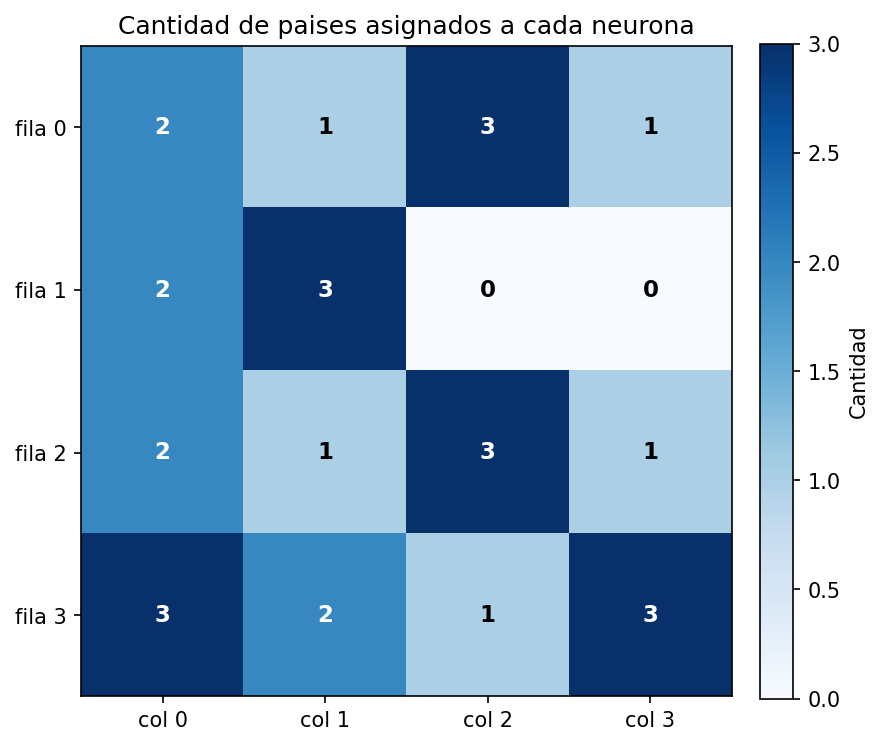
\includegraphics[width=\linewidth]{kohonen_hits_map}
    \end{column}
    \begin{column}{0.45\textwidth}
      \begin{itemize}
        \item 14 de 16 neuronas reciben al menos un pais.
        \item Maximo: 3 paises (varias neuronas).
        \item 2 neuronas vacias en la zona-frontera (col 2--3, fila 1) --- consistente con la Matriz U.
      \end{itemize}
      \vspace{0.5em}
      No hay neuronas ``muertas'' lejos de los datos: la inicializacion con muestras evita ese problema.
    \end{column}
  \end{columns}
\end{frame}

\begin{frame}{Mapas por variable: que significa cada zona}
  \centering
  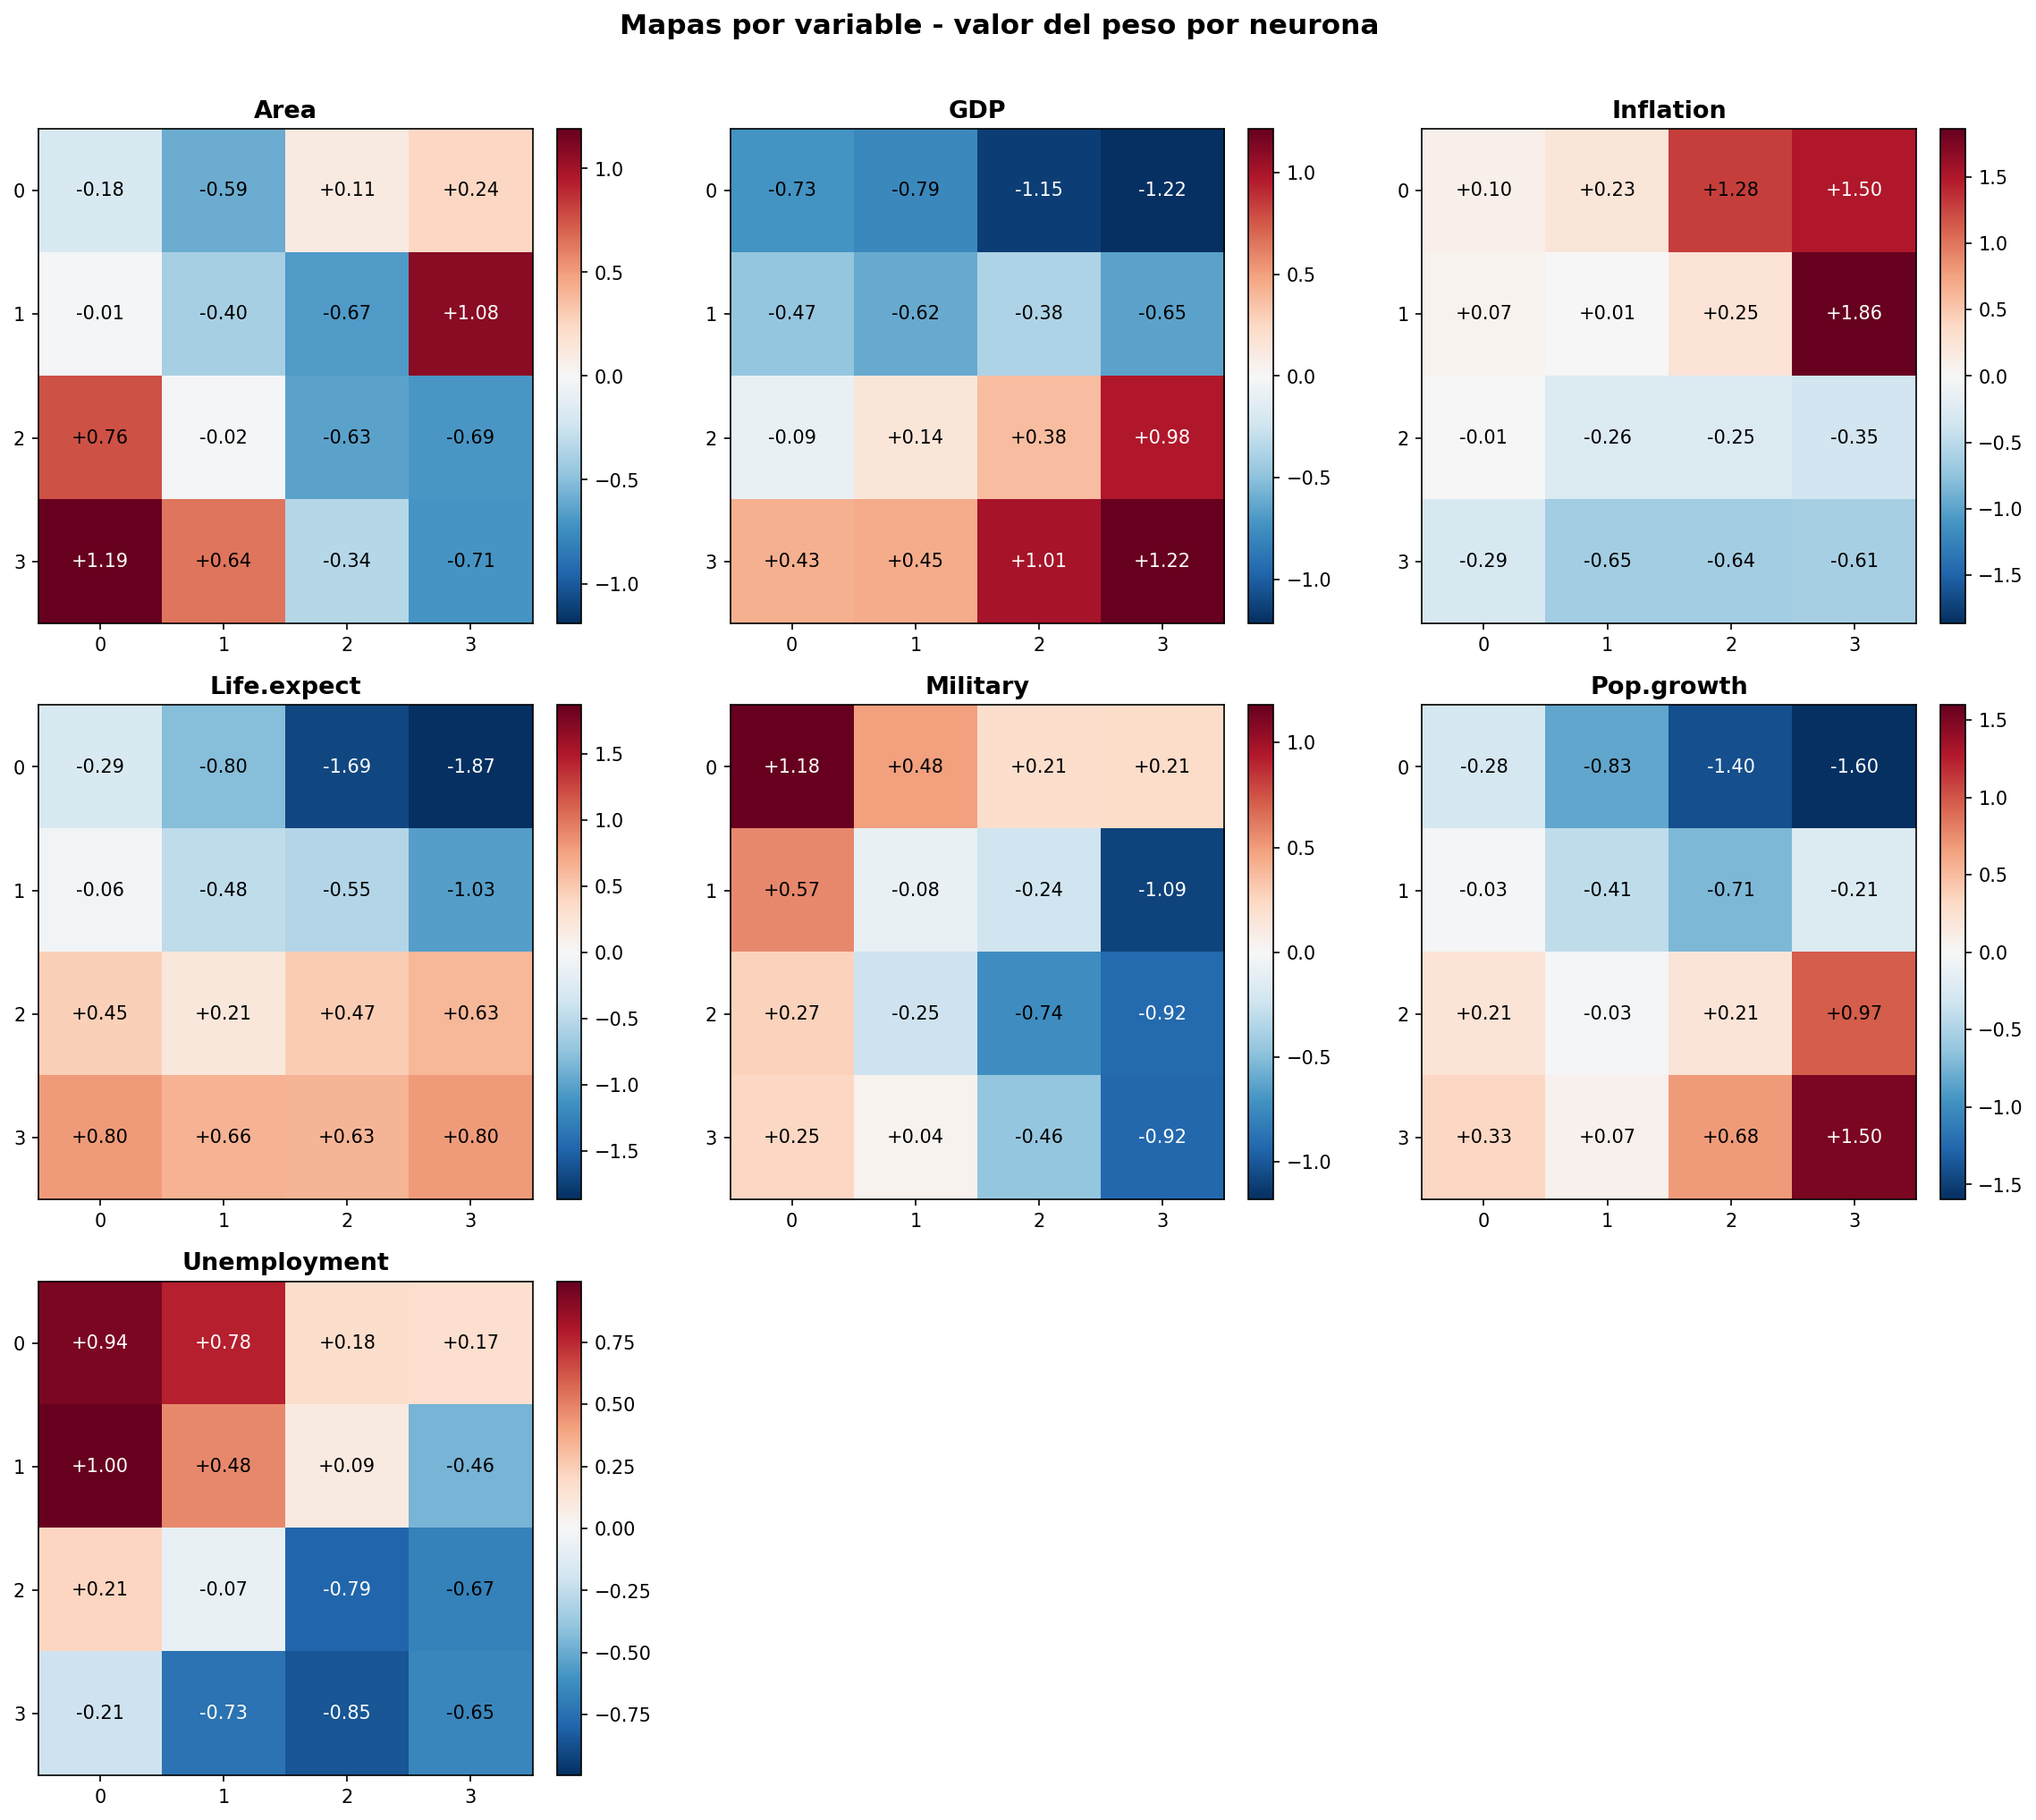
\includegraphics[height=0.85\textheight]{kohonen_variable_maps}
\end{frame}

\begin{frame}{Interpretacion del mapa}
  \begin{itemize}
    \item \textbf{Fila 3 (abajo)} --- alta \texttt{GDP}, alta \texttt{Life.expect}: Finland, Italy, Sweden, Germany, Norway, Netherlands, Ireland, Luxembourg, Switzerland.
    \item \textbf{Fila 0 (arriba)} --- baja \texttt{GDP}, alta \texttt{Inflation}, alta \texttt{Unemployment}: Croatia, Greece, Hungary, Bulgaria, Estonia, Latvia, Ukraine.
    \item \textbf{Columna 0 (izquierda)} --- alta \texttt{Military}: Grecia, Croacia, Spain.
    \item \textbf{Columna 3 esquina (0,3)} --- aislada por la Matriz U: Ucrania, $-$PIB, $+$inflacion extrema (8\%).
  \end{itemize}
  \vspace{0.5em}
  Los ejes ortogonales del SOM \textbf{coinciden con los ejes PC1 y PC2}:
  \begin{itemize}
    \item Vertical $\approx$ PC1 (desarrollo).
    \item Horizontal $\approx$ PC2 (crisis fiscal).
  \end{itemize}
\end{frame}

% ============================================================
% CIERRE
% ============================================================

\section{Conclusiones}

\begin{frame}{Que aprendimos del EJ1}
  \begin{itemize}
    \item \textbf{PC1 captura ``desarrollo / bienestar''} --- combinacion ponderada de $+$GDP, $+$Life.expect, $+$Pop.growth, $-$Inflation, $-$Unemployment. Explica el 46\% de la varianza.
    \item \textbf{Oja recupera PC1} sin resolver autovalores explicitamente: cosine similarity $0.99999943$, ranking de paises identico al de la libreria. Validacion total de la teoria iterativa.
    \item \textbf{El SOM produce un mapa topologico consistente con PCA}: paises del bloque oeste-norte vs este-sur, con Ucrania aislada como outlier. La Matriz U evidencia que el SOM aprende fronteras de cluster, no solo prototipos.
    \item Las tres tecnicas convergen al \alert{mismo relato geopolitico}: hay un eje principal de desarrollo y un eje secundario de crisis fiscal.
  \end{itemize}
\end{frame}

\begin{frame}[standout]
  Gracias.\\[0.6em]
  \small Codigo + figuras en el repositorio.
\end{frame}

\end{document}
